\documentclass[10pt,a4paper]{article}
\usepackage[utf8]{inputenc}
\usepackage{amsmath}
\usepackage{amsfonts}
\usepackage{graphicx}
\usepackage{subfigure}
\usepackage{amssymb}
\author{Oscar Daniel Juárez Cruz}
\title{Práctica 2}
\begin{document}
\maketitle
\section{Introducción}

\begin{flushleft}

Los procesos nos pueden ayudar a repartir varias tareas entre un número asinado de procesos. En esta ocasión usaremos procesos para multiplicar dos matrices de manera secuencial. \\ 
La multiplicación de matrices debe cumplir la siguiente condición \\ 
$ A_{axm} \cdot B_{mxb}  = M_{axb}$ \textit{el número de columnas de la matriz A es el número de filas de la matriz B y la matriz resultante M es de dimensiones axb}

\end{flushleft}

\begin{center}

\textbf{Multiplicación de matrices}

\end{center}

\begin{center}
	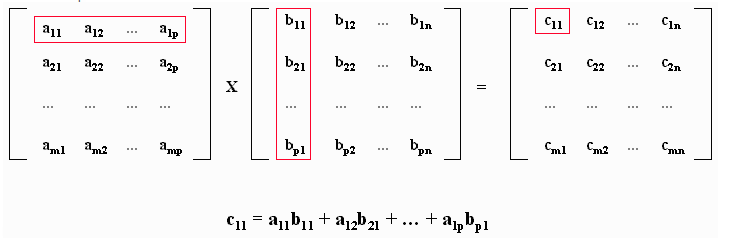
\includegraphics[scale=0.5]{mul.png}
\end{center}

\section{Desarrollo}

\begin{flushleft}
Reutilizamos parte del código anterior pero ahora en vez de que los hijos crearan más hijos iban a multiplicar dos matrices de manera distribuida, quiere decir que a cada proceso le corresponde multiplicar cierto número de filas e imprimirlas
\end{flushleft}

\begin{flushleft}
Para resolver el problema lo primero que debemos hacer es crear la matriz.
\end{flushleft}

\begin{flushleft}
Las matrices se crearon con memoria dinámica a traveś de la función crearMatriz(...).
\end{flushleft}

\begin{flushleft}
\textbf{int **crearMatriz(int nfilas, int ncolumnas)}
\end{flushleft}

\begin{center}
	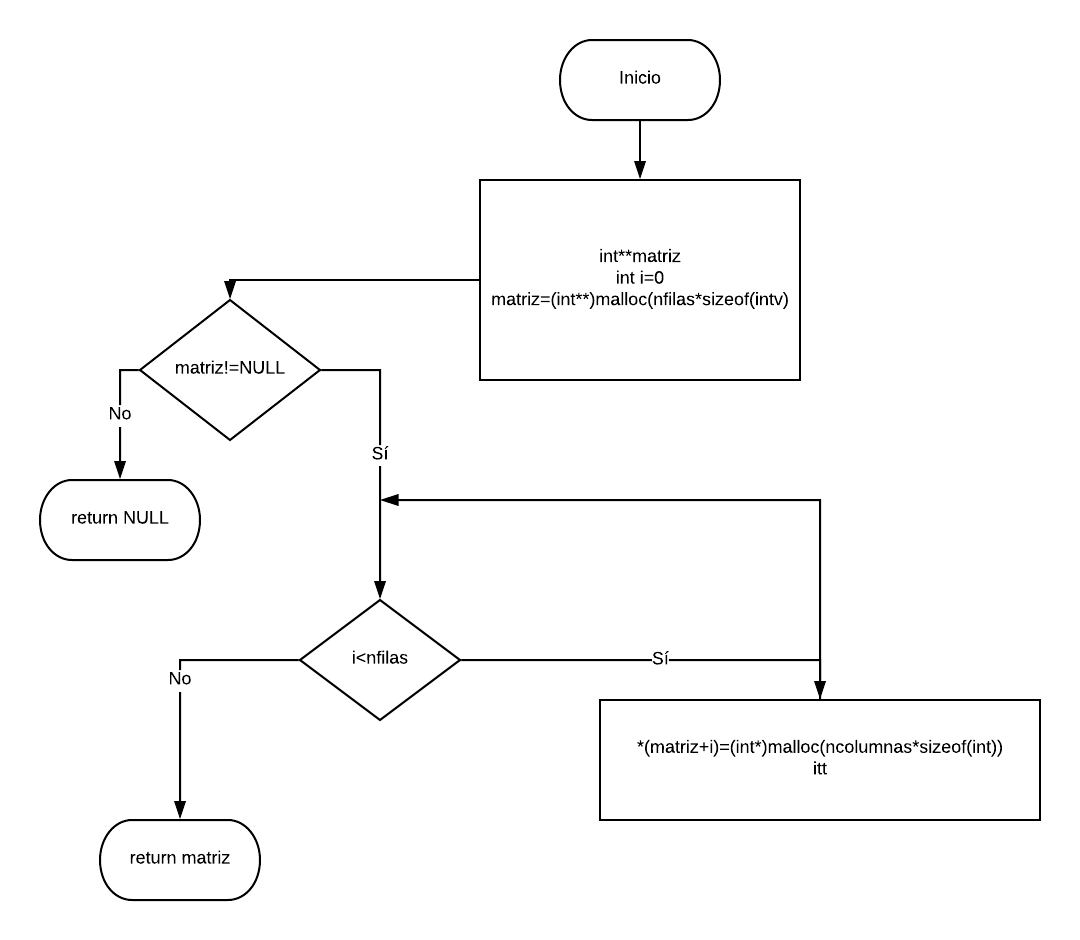
\includegraphics[scale=0.7]{crearMatriz.png} 
\end{center}

\begin{flushleft}
Después llenamos las matrices con la función llenarMatriz(...)
\end{flushleft}

\begin{flushleft}
\textbf{void llenarMatriz (int **matriz, int nfilas, int ncolumnas)}
\end{flushleft}

\begin{center}
	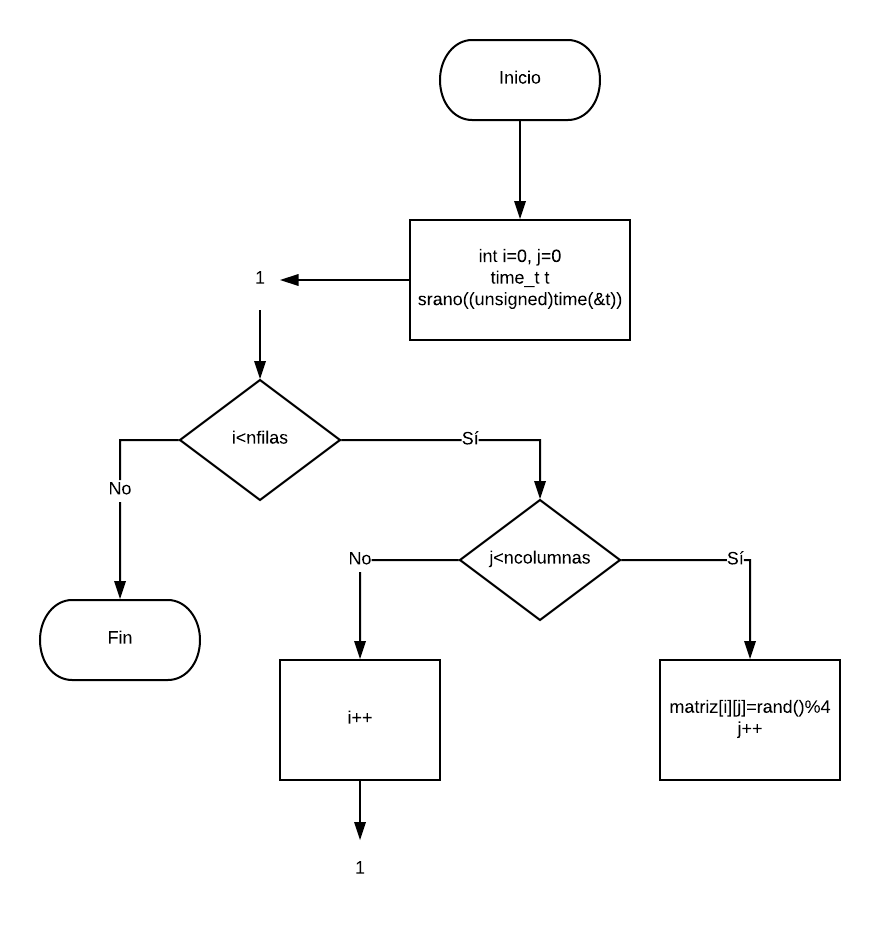
\includegraphics[scale=0.7]{llenarMatriz.png} 
\end{center}

\begin{flushleft}
Después mostramos las matrices creadas con la función imprimirMatriz(...)
\end{flushleft}

\begin{flushleft}
\textbf{void imprimirMatriz (int **m, int nf, int nc)}
\end{flushleft}

\begin{center}
	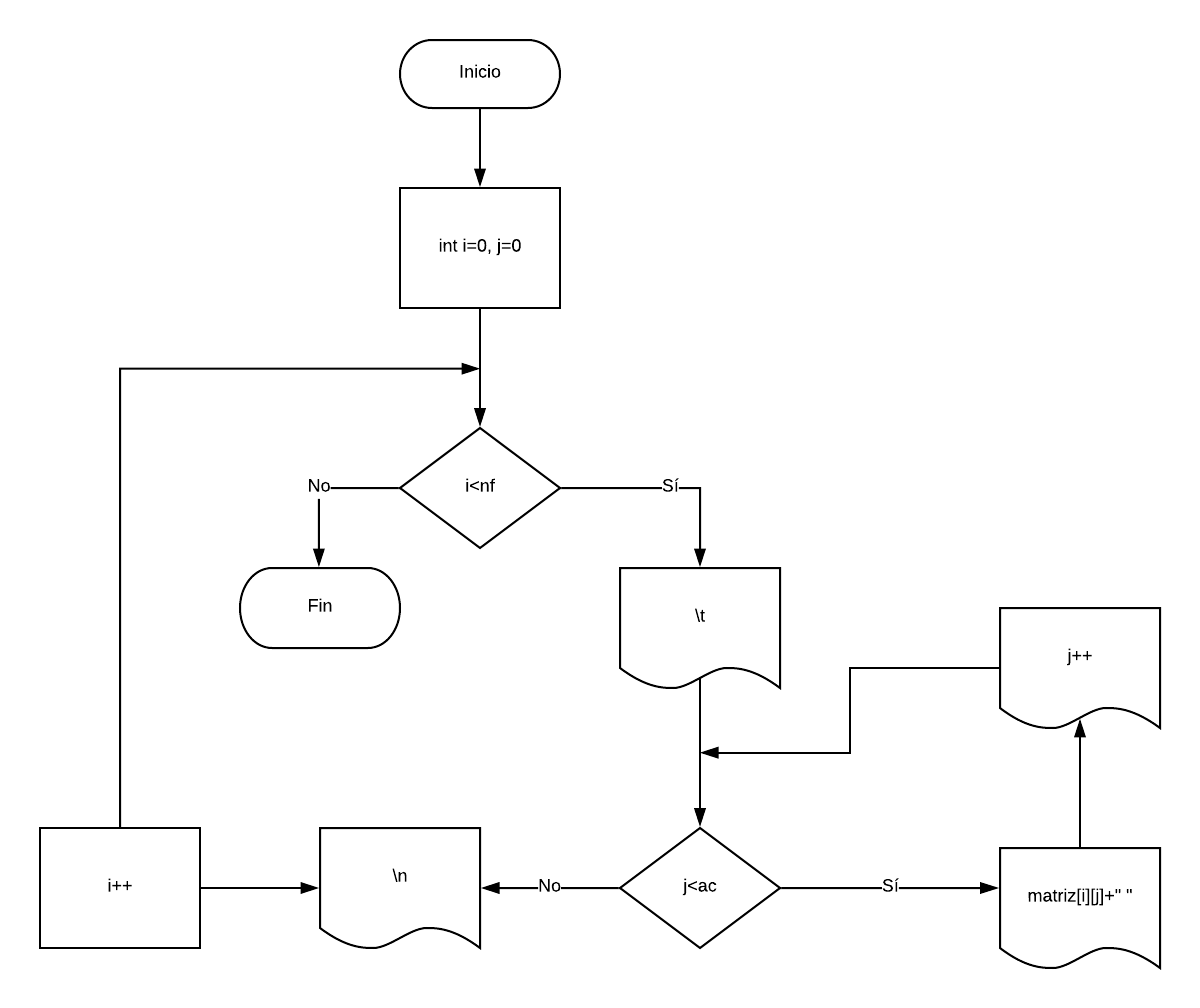
\includegraphics[scale=0.3]{imprimirMatriz.png} 
\end{center}

\begin{flushleft}
Elegimos el número de procesos que necesitamos y usamos la función dividirProcesos(...) para saber cuantas filas corresponden a cada hijo
\end{flushleft}

\begin{flushleft}
\textbf{void dividirProcesos(int *np, int *nfh, int *nfuh, int nf)}
\end{flushleft}

\begin{center}
	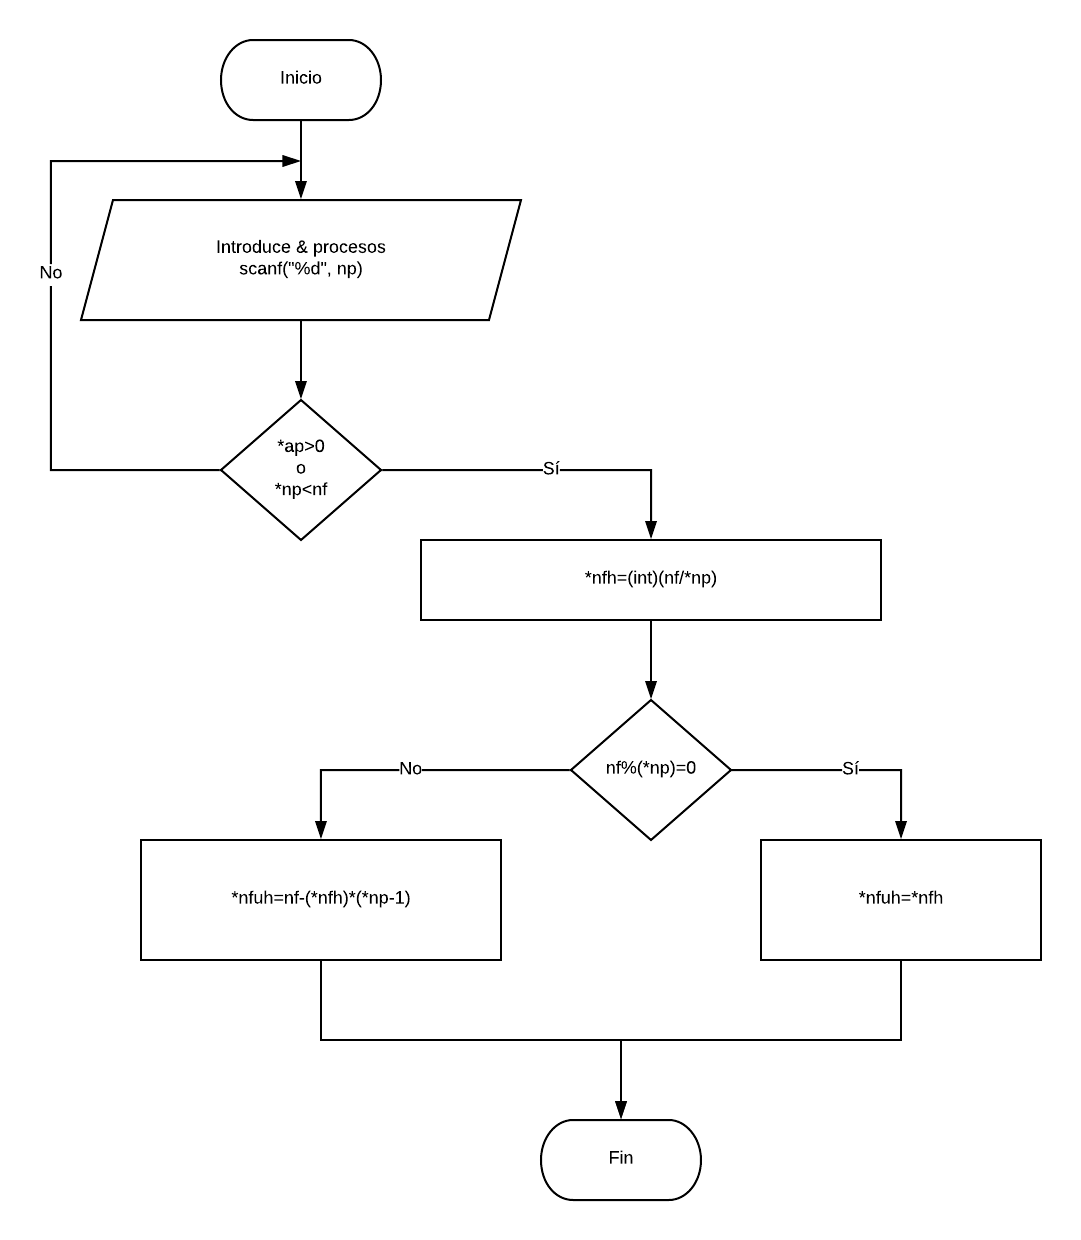
\includegraphics[scale=0.5]{dividirProcesos.png} 
\end{center}

\begin{flushleft}
Ahora creamos un for para poder iterar con los hijos y cada uno tiene la responsabilidad de multiplicar cierto número de filas con la función multiplicarMatrices(...)
\end{flushleft}

\begin{flushleft}
\textbf{void multiplicarMatrices (int **m1, int **m2, int rango, int id, int nf, int filas2, int columnas2)}
\end{flushleft}

\begin{center}
	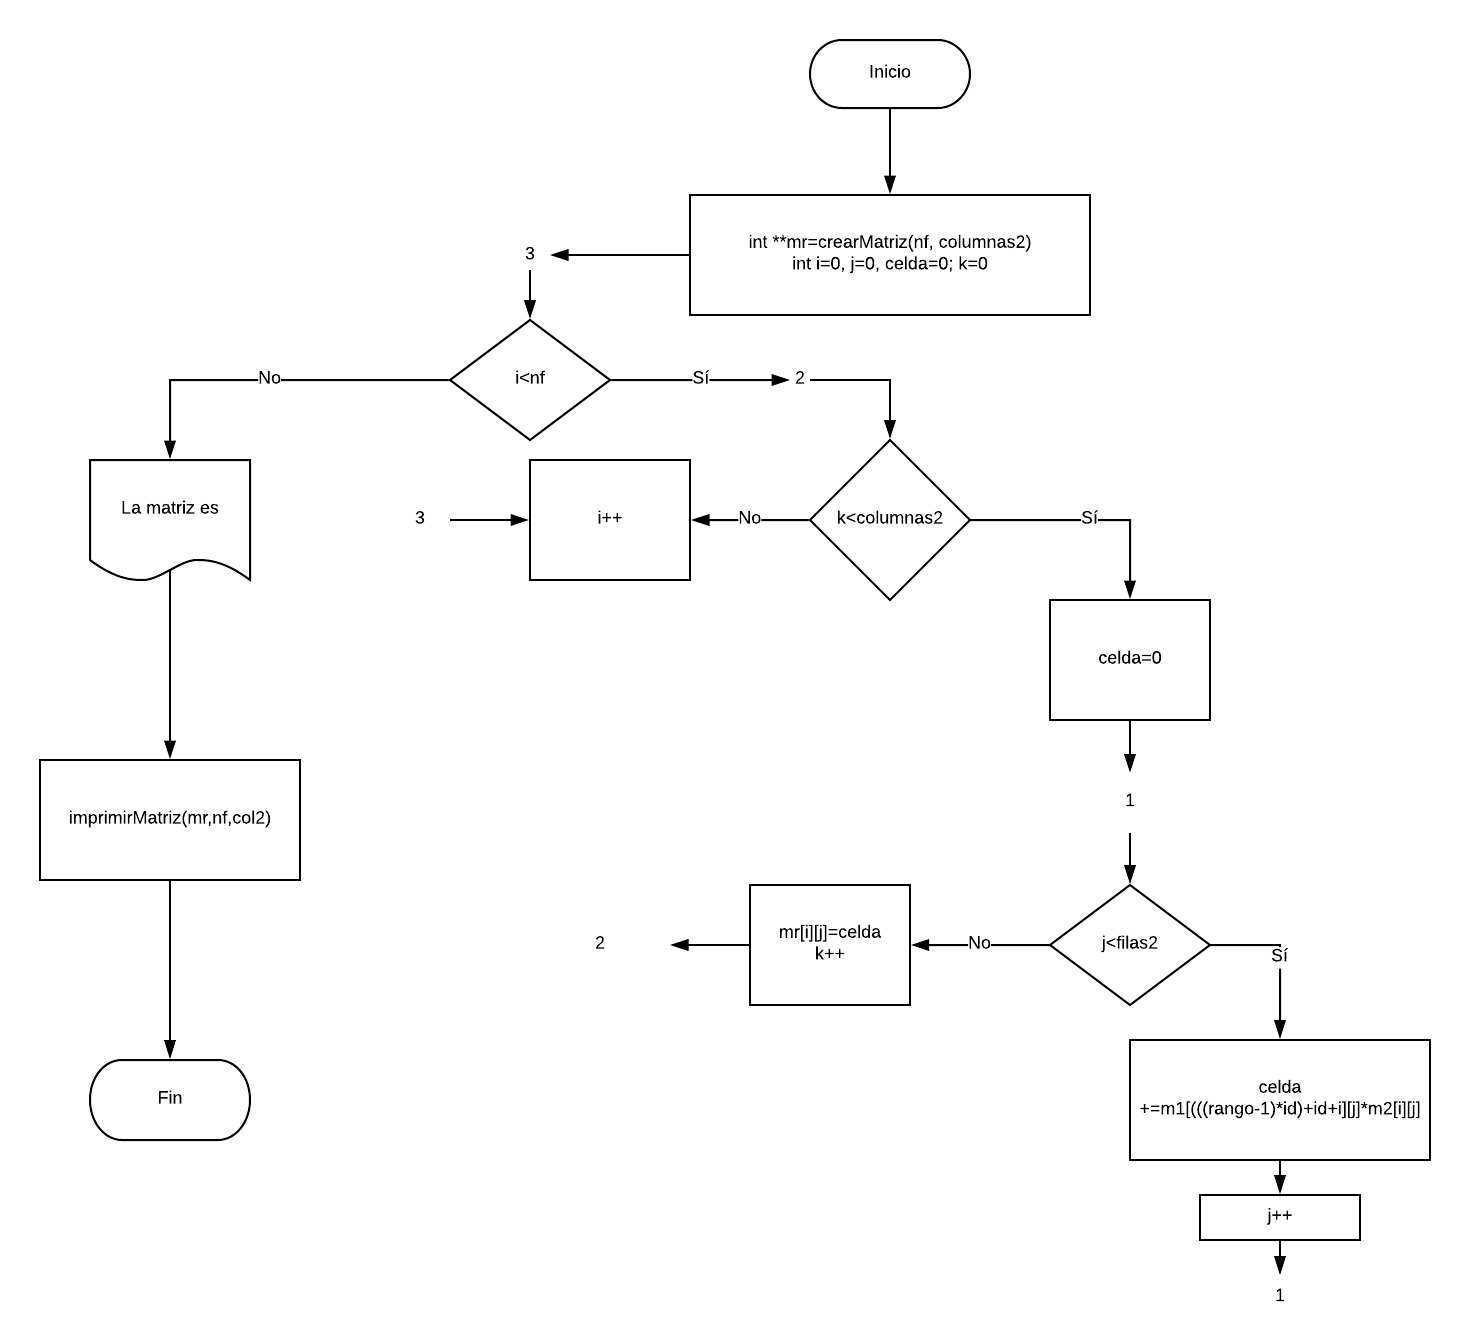
\includegraphics[scale=0.5]{multiplicarMatriz.png} 
\end{center}

\begin{flushleft}
Cada que se multiplica se va imprimiendo el número de proceso que la está haciendo y las filas correspondientes como se puede ver en el siguiente output
\end{flushleft}

\begin{flushleft}
	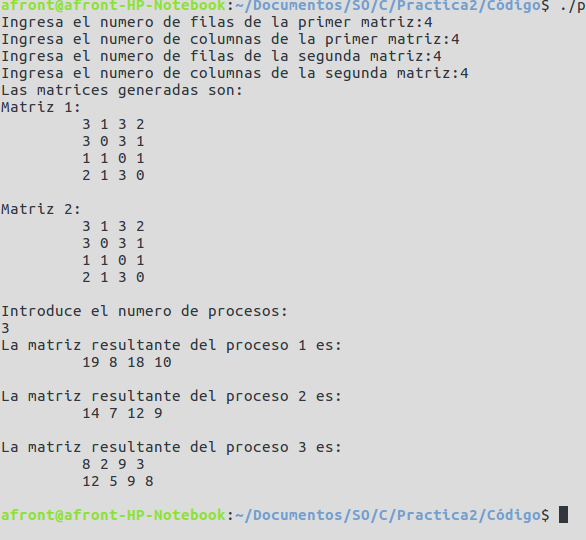
\includegraphics[scale=0.5]{screen.png} 
\end{flushleft}

\begin{flushleft}
	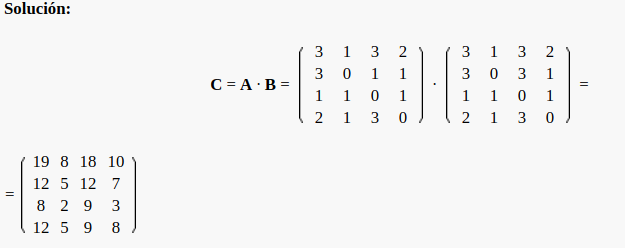
\includegraphics[scale=0.5]{screen1.png} 
\end{flushleft}

\section{Conclusión}

\begin{flushleft}
Los procesos nos pueden ayudar a optimizar una tarea repartiendola en varias, con lo que podemos generar un control sobre lo procesos cuando estos se ejecutan.
\end{flushleft}

\begin{flushleft}
Lo más complicado de la práctica fue hacer que la multiplicación se repartiera en diferentes procesos, pero al copiarse la información del padre a lo hijos ellos tenían el acceso a la matriz, pero aún así fue complicado generar la multiplicación y que cada hijo aportara una fila diferente
\end{flushleft}

\end{document}